\chapter{The \fshark{} language}
\textbf{test test}
In this chapter we present the \fshark{} language and it's standard library.
We start out by presenting \fshark{}'s syntax and discussing the syntax's
limitations.
Afterwards we present first the built-in \fsharp{} operators and \fsharp{}
standard library functions available in \fshark{}.
We then present our own standard library written specifically for \fshark{}, and
discuss why we implemented our own standard library instead of using the
standard library already available in \fsharp{}.

Then, we discuss how array types are implemented in \fshark{}, and how
\fsharp{} arrays differ from Futhark arrays.
Finally, we describe and solve the implementation challenges caused by our
design choices, and discuss alternative solutions to the one that was chosen.

\section{What the \fshark{} language is}
\label{chap:fsharklanguage}
The second contribution of this thesis is a high level programming language,
which can be compiled automatically to GPU kernels that are readily usable in
a mainstream programming language.

The \fshark{} language is the sum of two parts: \\
1) The \fshark{} subset, which is a defined subset of the \fsharp{} language and
the \fsharp{} standard library.\\
2) An accompanying standard library, which adds SOACs and array functions that
can be used in programs written in the \fshark{} subset.

The \fshark{} language can be compiled into standalone GPU kernels using the
\fshark{} compiler \ref{chap:fsharkcompiler}. These kernels can then be integrated directly in
\fsharp{} programs.

The program in figure \ref{fig:shortfsharkprogram0'} is written in \fshark{},
and can be used as any other \fsharp{} code in an \fsharp{} project.
However, as it is written in \fshark{}, we can pass it through the \fshark{}
compiler and end up with the result Futhark code shown in figure \ref{fig:shortfsharkprogram1'}
At this moment we we will skip explaining the meaning of the code, and simply
point out that the \fshark{} source code and the resulting source code have a
strong resemblance.
\begin{figure}[H]
  \centering
\begin{minted}{fsharp}
let saxpy (a : int) (x : int) (y : int) : int =
  a*x+y

let getArrayPair (a : int) : (int array * int array) =
  let xs = Iota a
  let n = Length xs
  let ys = Rotate (a / n) xs
  in (xs, ys)

[<FSharkEntry>]
let entry (a : int) : int array =
  let (xs, ys) = getArrayPair a
  let res = Map2 (saxpy a) xs ys
  in res
\end{minted}
  \caption{A short \fshark{} program}
  \label{fig:shortfsharkprogram0'}
\end{figure}

\begin{figure}[H]
  \centering
  \begin{lstlisting}[language=Futhark, breaklines]
let saxpy (a : i32) (x : i32) (y : i32) : i32 =
  ((((a * x)) + y))
let getArrayPair (a : i32) : ([]i32, []i32) =
  let xs = iota (a)  in
  let n = length (xs)  in
  let ys = rotate (((a / n))) (xs) in
  (xs, ys)
entry entry (a : i32) : []i32 =
  unsafe let patternInput = getArrayPair(a) in
         let ys = patternInput.2 in
         let xs = patternInput.1 in
         let res = map2 ((\(x : i32) -> (\(y : i32) -> saxpy(a) (x) (y)))) (xs) (ys) in
         res
\end{lstlisting}
  \caption{The source code in figure \ref{fig:shortfsharkprogram0'} compiled to
    Futhark source code by the \fshark{} compiler.}
  \label{fig:shortfsharkprogram1'}
\end{figure}

In the following section, we will describe the entire \fshark{} language. Although the
subset is just a part of \fsharp{}, we will describe it as if it was a new language.

\clearpage
\section{\fshark{} syntax}
\Cref{fig:fsharkstatements,fig:fsharkexpressions,fig:fsharkpatterns,fig:fsharktypes,fig:fsharkliterals}
shows the complete \fshark{} syntax.

\begin{figure}[h]
  \centering
  \begin{tabular}{lclr}
    $prog$ & $::=$ & $module\ prog$ & \\
           & $|$   & $prog'\ prog$  & \\
           & $|$   & $\epsilon$     & \\

    $prog'$ & $::=$ & $typealias$   & \\
            & $|$   & $fun$ & \\

    $progs'$ & $::=$ & $prog'\ progs'$   & \\
             & $|$   & $\epsilon$ & \\
    \\
    $typealias$ & $::=$ & $\texttt{type}\ v\ = t $& \\
    $module$ & $::=$ & $\texttt{module}\ v = prog'\ progs'$ & \textit{(See subsec \ref{noteonfsharkmodules} on \fshark{} modules)} \\
    \\
  \end{tabular}
  \begin{tabular}{lclr}
    $fun$ & $::=$ & \texttt{[<FSharkEntry>]} $\texttt{let}\ id\ (v_1 : t_1)\ \ldots\ (v_n : t_n) : t = e$ & \\
        & $|$   & $\texttt{let}\ v\ (v_1 : t_1)\ \ldots\ (v_n : t_n) : t' = e,$ & \textit{{See subsec \ref{noteonfsharktypes}}}  \\
    \\

  \end{tabular}
  \caption{\fshark{} statements}
  \label{fig:fsharkstatements}
\end{figure}



\begin{figure}[h]
  \centering
  \begin{tabular}{lclr}
    $e$ & $::=$ & $(e)$ & (Expression in parenthesis) \\
        & $|$   & $k$ & (Constant) \\
        & $|$   & $v$ & (Variable) \\
        & $|$   & $(e_0,~\ldots,~e_n)$ & (Tuple expression) \\
        & $|$   & $\{\texttt{id}_0=e_0 ; \ldots ; \texttt{id}_n=e_n\}$ & (Record expression) \\
        & $|$   & $[\vert e_0 ; \ldots ; e_n\vert]$ & (Array expression) \\
        & $|$   & $v.[e_0] \ldots .[e_n]$ & (Array indexing) \\
        & $|$   & $v.id$ & (Record indexing) \\
        & $|$   & $v.id$ & (Module indexing (\textit{See subsec \ref{noteonfsharkmodules}})) \\
        & $|$   & $e_1 \odot e_2$ & (Binary operator) \\
        & $|$   & $-e$ & (Prefix minus) \\
        & $|$   & \texttt{not} $e$ & (Logical negation) \\
        & $|$   & \texttt{if} $e_1$ \texttt{then} $e_2$ \texttt{else} $e_3$ & (Branching) \\
        & $|$   & \texttt{let} $p = e_1$ \texttt{in} $e_2$ & (Pattern binding) \\
        & $|$   & $\mathtt{fun}~p_0~\ldots~p_n~\mathtt{->}~e$ & (Anonymous function) \\
        & $|$   & $e_0~e_1$ & (Application) \\

    \\
  \end{tabular}
  \caption{\fshark{} expressions}
\label{fig:fsharkexpressions}
\end{figure}

\begin{figure}[h]
  \centering
  \begin{tabular}{@{}lclr}
    $p$ & $::=$ & $id$ & (Name pattern) \\
        & $|$   & $(p_0, \ldots, p_n)$ & (Tuple pattern) \\
  \end{tabular}
  \caption{\fshark{} patterns}
\label{fig:fsharkpatterns}
\end{figure}



\begin{figure}[h]
  \centering
  \begin{tabular}{@{}lclr}
    $t$ & $::=$ & $\texttt{int8}~|~\texttt{int16} ~|~ \texttt{int} ~ |~\texttt{int64} $ & (Integers) \\
        & $|$   & $\texttt{uint8} ~ | ~\texttt{uint16} ~|~\texttt{uint} ~|~\texttt{uint64} $ & (Unsigned integers) \\
        & $|$   & $\texttt{single} ~| ~\texttt{double}$ & (Floats) \\
        & $|$   & $\texttt{bool}$ & (Booleans) \\
        & $|$   & $(t_0 * \ldots * t_n)$ & (Tuples) \\
        & $|$   & $\{id_0:t_0;~\ldots;~id_n:t_n\}$ & (Records) \\
        & $|$   & $t~\mathtt{array}$& (Arrays) \\
    \\
  \end{tabular}
  \caption{\fshark{} types}
\label{fig:fsharktypes}
\end{figure}

\begin{figure}[h]
  \centering
  \begin{tabular}{@{}lclr}
    $k$ & $::=$ & $n\lit{y}~|~n\lit{s}~|~n~|~n\lit{L}$ & (8-, 16-, 32- and 64 bit signed integers) \\
        & $|$   & $n\lit{uy}~|~n\lit{us}~|~n~|~n\lit{UL}$ & (8-, 16-, 32- and 64 bit unsigned integers) \\
        & $|$   & $d\lit{f}~|~d $ & (Single and double precision floats) \\
        & $|$   & $true~|~false$ & (Boolean) \\
        & $|$   & $(k_0 ,~\ldots ,~k_n)$ & (Tuple) \\
        & $|$   & $\{id_0=k_0;~\ldots;~id_n=k_n\}$ & (Record) \\
        & $|$   & $[\vert k_0 ; \ldots ; k_n\vert]$ & (Array literals) \\
    \\
  \end{tabular}
  \caption{\fshark{} literals}
\label{fig:fsharkliterals}
\end{figure}
\clearpage
\section{Notes to the \fshark{} grammar}
\subsection{Limits to function argument types}
\label{noteonfsharktypes}
There are several limits to the \fsharp{} compiler, which limits the types
available in function definitions.\\
\begin{enumerate}
\item Tuples in entry functions, whether they are used in the arguments or in the
return types, are allowed to contain a maximum of seven elements. This is
because the CLR runtime uses the type \texttt{System.Tuple} for these tuples.
Incidentally, \texttt{System.Tuple} is only defined for tuples up to seven
elements.

This limitation can be circumvented by using more tuples. For example, rewriting
a function so it returns \\
\texttt{((int * int * int * int) * (int * int * int * int))}\\
instead of\\
\texttt{(int * int * int * int * int * int * int * int)}.

\item Non-entry functions cannot have tuple type arguments.
  For functions that take tuple arguments, the \fsharp{} compiler parses these
  tuple type arguments correctly.
  However, the \fsharp{} compiler rewrites calls to these functions in a curried
  way. Figure~\Cref{fig:astcurried} shows two two \fsharp{} functions, {\tt foo}
    and {\tt bar}, and figure~\Cref{fig:astcurried'} shows a simplified 
    representation of how these functions are represented in the
    \fsharp{}-compiler intermediate representation.

  When translating from \fshark{} to Futhark, the Foo function is correctly
  written in Futhark as a function with a tuple argument, but since the call
  expression {\tt Call foo 4 5} now treats \texttt{foo} as having a different 
  type than first defined, the corresponding Futhark translation will trigger 
  a type error at compile time.

\begin{figure}[H]
\centering
\begin{minted}{fsharp}
let foo ((x , y) : (int * int)) : int = x + y

let bar = foo (4,5)
\end{minted}
\caption{A function calling another function in \fsharp{}}
    \label{fig:astcurried}
    \end{figure}
\begin{figure}[H]
\begin{minted}{lisp}
Function foo ((x , y) : (int * int)) : int = x + y

Function bar () : int = Call foo 4 5
\end{minted}
    \caption{\fsharp{} compiler curries tuple arguments when calling tuple functions}
    \label{fig:astcurried'}
  \end{figure}

\item Entry functions should not use record type arguments, as these have not
  been investigated fully for \fshark{} use yet.
\end{enumerate}

\subsection{\fshark{} modules}
\label{noteonfsharkmodules}
The modules supported in \fshark{} are not higher-order modules as in
\texttt{ML}, but instead just a nested namespace in the containing module.

\section{\fsharp{} operators available in \fshark{}}
The \fsharp{} subset chosen for \fshark{} is described in \ref{fig:fsharkops}.
Note that all of these operators are overloaded and defined for all integer
and floating point types in \fsharp{}, except for modulus which in Futhark is
only defined for integers.

\begin{figure}[h]
  \centering
\begin{description}
\item[Arithmetic operators]\hfill\\
  The set of supported arithmetic operators is addition (\texttt{+}),
  binary subtraction and unary negation (\texttt{-}), multiplication
  (\texttt{*}), division (\texttt{/}) and modulus (\texttt{\%}).

\item[Boolean operators]\hfill\\
  \fshark{} currently supports logical AND (\texttt{\&\&}), logical OR
  (\texttt{$||$}), less- and greater-than (\texttt{<}, \texttt{>}), less- and
  greater-or-equal (\texttt{<=}, \texttt{>=}), equality (\texttt{=}),
  inequality (\texttt{<>}) and logical negation (\texttt{not}).

\item[Special operators]\hfill\\
  \fshark{} also supports some of \fsharp{}s syntactic sugar. These operators
  might not have direct Futhark counterparts, but their applications can be
  rewritten in Futhark for equivalent functionality.
  The supported operators are back- and forward pipes (\texttt{<|} and
  \texttt{|>}), and the range operator ($e_0$ \texttt{..} $e_1$), which
  generates the sequence of numbers in the interval $[e_0,e_1]$.

  Note that the range operator must be used inside an array (as so
  \texttt{$[\vert e_0..e_1\vert]$}), so the expression generates an array
  instead of a list.
\end{description}
  \caption{\fshark{} operators}
\label{fig:fsharkops}
\end{figure}



\section{\fsharp{} standard library functions available in \fshark{}}
\fshark{} supports a subset of the \fsharp{} standard library. These are
readily available in all \fsharp{} programs, without having to open other modules.
The standard library subset is shown in figure \ref{fig:fsharkfuns}.
\begin{figure}[h]
  \centering
\begin{description}
\item[\texttt{id}]\hfill\\
  The identity function.

\item[Common math function]\hfill\\
  The square root function (\texttt{sqrt}), the absolute value (\texttt{abs}),
  the natural exponential function (\texttt{exp}), the natural- and the decimal
  logarithm (\texttt{log} and \texttt{log10}).
  
\item[Common trigonometric functions]\hfill\\
  Sine, cosine and tangent functions (both standard and hyperbolic):
  \texttt{sin}, \texttt{cos}, \texttt{tan}), \texttt{sinh}, \texttt{cosh} and \texttt{tanh}.
  Also one- and two-argument arctangent: \texttt{atan} and \texttt{atan2}.

\item[Rounding functions]\hfill\\
  \fshark{} supports all of \fsharp{}s rounding functions:
  \texttt{floor}, \texttt{ceil}, \texttt{round} and \texttt{truncate}.
  
\item[Number convertion functions]\hfill\\
  \fshark{} supports all of \fsharp{}s number convertion functions.
  For all the following functions $t$, $t e = e', e : t_0, e' : t$, barring
  exceptions like trying to convert a too large 64-bit integer into a 32-bit
  integer.

  The convertion functions available are \texttt{int8}, \texttt{int16}, \texttt{int}, \texttt{int64}, \texttt{uint8}, \texttt{uint16},
  \texttt{uint}, \texttt{uin64}, \texttt{single}, \texttt{double}, \texttt{bool}.
  
\item[Various common number functions]\hfill\\
  \texttt{min}, \texttt{max}, \texttt{sign} and \texttt{compare}.
\end{description}
  \caption{\fshark{} operators}
  \label{fig:fsharkfuns}
\end{figure}

\subsection{On selection the \fsharp{} subset to include in \fshark{}}
For selecting the \fsharp{} subset to support in \fshark{}, I chose to look at
what functions that were included in \fsharp{}'s prelude. That is, the
functions that are available in an \fsharp{} program without having to
\texttt{open} their containing module first.
Fortunately, \fsharp{} opens several modules by default of which I only
needed to look in two different ones, to be able to support a reasonable amount
of \fsharp{} built-ins in \fshark{}.

The primary module used in my supported \fsharp{} subset is the module
\texttt{FSharp.Core.Operators}.
This module contained not only the standard arithmetic described in figure
\ref{fig:fsharkops}, but also most\footnote{except for some convertion
  functions, found in \texttt{FSharp.Core.ExtraTopLevelOperators}} of the functions shown in the figure \ref{fig:fsharkfuns}.
Except for \texttt{unit} type functions like \texttt{failwith}, \texttt{exit}
and \texttt{async}, most of the functions and operators
\texttt{FSharp.Core.Operators} have direct counterparts in Futhark's prelude,
with equivalent functionality: All except for four of operators and functions chosen for
\fshark{} are in fact implemented in Futhark's \texttt{math.fut} library.
It was therefore an obvious decision to support these functions and operators in
\fshark{}.

However, for the remaining four functions\footnote{\texttt{compare}, \texttt{cosh}, \texttt{sinh}, \texttt{tanh}} that didn't have equivalents in
Futhark's \texttt{math.fut}, their function calls are replaced with their
identities instead.
For example, the \fshark{} code shown below:
\begin{minted}{fsharp}
  exp x
\end{minted}

can be expressed in Futhark directly as shown below:
\begin{lstlisting}[language=Futhark]
  exp x
\end{lstlisting}

However, the hyperbolic cosine function (shown below) is available in \fsharp{}, but not in Futhark.
\begin{minted}{fsharp}
  cosh x
\end{minted}
Therefore, the compiled \fshark{} Futhark code is just the hyperbolic function
inlined.
When the \fshark{} compiler encounters the \texttt{cosh} function the \texttt{cosh} call is replaced with
  \texttt{cosh}'s definition in the \fshark{} generated Futhark code. This is
  shown below:
  
\begin{lstlisting}[language=Futhark]
  ((exp x) + (exp (-x))) / 2.0
\end{lstlisting}

These rewritings are not pretty to look at from a programmer's perspective, but
the Futhark code generated by the \fshark{} compiler is not meant to be read by humans anyhow.

\subsection{Missing arithmetic operators in \fshark{}}
Currently, bitwise operators like bitwise-AND and bitwise-OR are missing, but
they should be relatively simple to add to the \fshark{} subset, by adding them
to the set of supported operators in the \fshark{} compiler.

\section{The \fshark{} standard library}
Besides defining an \fsharp{} subset suitable for Futhark translation, it was
also imperative to create a standard library of SOACs and array functions for \fshark{},
to make it possible to write programs with parallel higher-order array
functions.
\\
We call this standard library \texttt{FSharkPrelude}.

Similarly to how the subset of math functions chosen from \fsharp{} to include in
the \fshark{} was chosen, the SOACs and array function included in the
\texttt{FSharkPrelude} has been picked directly from the Futhark libraries
\texttt{futlib/array.fut} and \texttt{futlib/soacs.fut}. The \texttt{FSharkPrelude} doesn't
discriminate between array functions and SOACs, as maintaining and importing two
different prelude files in \fshark{} was needlessly complicated.

The \texttt{FSharkPrelude} consists of functions which are directly named after
their Futhark counterparts, and have equivalent functionality.
This prelude, together with the \fshark{} subset, is what makes up the \fshark{} language.
When \fshark{} developers are writing modules in \fshark{}, they are "guaranteed"
that their \fshark{} programs has the same results whether they are executed as
native \fsharp{} code, or compiled and executed as Futhark. 
The guarantee is on the condition that we know that the
individual parts of the \fshark{} language and standard library,  are correctly
translated to Futhark counterparts.
We can check that this condition still holds by running the \fshark{} test
suite. See sec \ref{subsec:fsharkcorrectness} for an elaboration on these tests.


The \texttt{FSharkPrelude} versions of Futhark functions are defined in three
different ways.
\begin{enumerate}
  \item Functions like \texttt{map} and array functions like
    \texttt{length} have direct \fsharp{} equivalents. The
    \texttt{FSharkPrelude} versions therefore simply pass their arguments on to
    the existing functions.
    Other functions, like the \texttt{map} functions which takes multiple arrays as
    arguments, require a bit of assembly first. For those \texttt{map} functions,
    we zip the arguments before using \texttt{Array.map} as usual.
    For example, FSharkPrelude.Map, -Map3 and -Map4 are shown below:
\begin{minted}{fsharp}
let Map (f : 'a -> 'b) (xs : 'a array) : 'b array =
  Array.map f xs

let Map3 f aa bb cc =
    let curry f (a,b,c) = f a b c
    let xs = Zip3 aa bb cc
    in Array.map (curry f) xs

let Map4 f aa bb cc dd =
    let curry f (a,b,c,d) = f a b c d
    let xs = Zip4 aa bb cc dd
    in Array.map (curry f) xs
\end{minted}

  \item Some Futhark SOACs have \fsharp{} counterparts that are very close to
    their original definition.
    for example, Futhark's \texttt{reduce} takes a neutral element\footnote{For
      parallelization purposes} as one of the
    arguments in their function calls, whilst their \fsharp{} counterparts
    (\texttt{Array.reduce}) does only take an operator and an array as
    arguments.
    In such cases, the \texttt{FSharkPrelude} version changes the input slightly
    before passing it on to the existing function. See example below:

\begin{minted}{fsharp}
let Reduce (op: 'a -> 'a -> 'a) (neutral : 'a) (xs : 'a array) =
  if null xs then neutral 
  else Array.reduce op xs
\end{minted}

  \item Lastly, some functions does not have \fsharp{} counterparts at all, such
    as scatter. In these cases, we manually implement an equivalent function in
    \fsharp{}.
    Note that we are not limited to the \fshark{} subset in the
    \texttt{FSharkPrelude}, as the prelude function calls are not translated by the
    \fshark{} compiler, but detected and exchanged for
    Futhark function calls of the same name during the \fshark{} compilation.
    \texttt{FSharkPrelude.Scatter}\footnote{The SOAC Scatter actually has limitations
      regarding \fshark{} use. See section~\ref{subsec:badscatter}} is shown below:
\begin{minted}{fsharp}
let Scatter (dest : 'a array) (is : int array) (vs : 'a array) : 'a array =
  for (i,v) in Zip is vs do
    dest.[i] <- v
  dest
\end{minted}

\end{enumerate}
The complete list of available SOACs and array functions is available in
appendix \ref{appendix:soacs}.

\subsection*{Why is FSharkPrelude part of the \fshark{} language?}
Although plenty of functions in the Futhark library already has \fsharp{}
counterparts, we have chosen not to allow these \fsharp{} counterparts to be
used directly in \fshark{} programs.
Besides basic differences like different naming in \fsharp{} and Futhark for
equivalent functions\footnote{like \texttt{fold} and \texttt{foldBack} vs.
  \texttt{foldl} and \texttt{foldr}} like, there are multiple other reasons.

1) From a user experience point of view, it is awkward to maintain a whitelist
of accepted functions from certain classes.
For example, \texttt{Array.map} is exchangable with Futhark's
\texttt{map}, but there are no immediate Futhark version of \fsharp{}s
\texttt{Array.sortInPlace}. Therefore, the \fshark{} compiler would succesfully
exchange a call to \texttt{Array.map} with a call to \texttt{map}, but it would
have to halt with an error message, if the user tried to use \texttt{Array.sortInPlace}.

2) Some Array functions have subtle differences compared to their
Futhark counterparts. As shown in \texttt{FSharkPrelude.Reduce} example,
\texttt{Array.reduce} is slightly different in \fsharp{}.

We are slightly hypocritical, as we DO let users use a subset of \fsharp{}s
standard library functions. However, there is a whitelist available for this
subset in the \fshark{} language specification, and the standard library
functions are not visibly called as a method from another module.

\subsection*{How \fshark{} SOACs differ from Futhark's ditto}
On a surface level, \fshark{} and Futhark SOACs are the same. After all, they
have equivalent functionality.
However, Futhark's SOACs gets special treatment in the Futhark compiler, and are
fused together where applicable.
Take for instance the short code example in figure \ref{fig:futharkfusion}.

\begin{figure}[h]
  \centering
\begin{lstlisting}[language=Futhark]
entry main : []f32 =
  let xs = iota 100
  let ys = map (f32.i32) xs
  let zs = map (+ 4.5f32) ys
  in zs
\end{lstlisting}
  \caption{A short Futhark program consisting of just SOACs}
  \label{fig:futharkfusion}
\end{figure}

For non-OpenCL programs, Futhark's compiler fuses all three expressions into one for-loop, as described
in simplified Futhark \csharp{} code in figure \ref{fig:pseudofusion}.
Similarly, in an OpenCL program, the short code example is translated into a
single kernel, as shown in figure \ref{fig:pseudokernel}.

\begin{figure}[h]
  \centering
\begin{minted}{csharp}
float[] mem = new float[100];
for (int i = 0 ; i < 100 ;i++)
{
  float res = int_to_float(i);
  res = res + 4.5f;
  mem[i] = res;
}
\end{minted}
  \caption{Figure \ref{fig:futharkfusion} compiled as (simplified) non-OpenCL
    \csharp{} code.}
  \label{fig:pseudofusion}
\end{figure}

\begin{figure}
  \centering
\begin{minted}{cpp}
__kernel void map_kernel(__global unsigned byte *mem)
{
   int global_thread_id = get_global_id();
   bool thread_active = global_thread_id < 100;

   float res;

   if (thread_active) {
       res = int_to_float(global_thread_id);
       res = res + 4.5f;
   }
   if (thread_active) {
       *(__global float *) &mem[global_thread_id * 4] = res;
   }
};
\end{minted}
  \caption{Figure \ref{fig:futharkfusion}, but compiled as a simplified OpenCL kernel.}
  \label{fig:pseudokernel}
\end{figure}


In both of the compiled examples, we must first allocate a target array for our
result, but note that although we obtain three different arrays in the original
Futhark code, both of the compiled versions transform the \texttt{iota}
expression into a for-loop instead, and inserts the operators from the two
subsequent \texttt{map}s into the loop.

This is a concrete implementation Futhark fusion rules as defined in \cite{pldi17}; which states
that $(map~f) \circ (map~g) \equiv map (f \circ g)$

However, executing \fshark{} code as native \fsharp{} code will execute the
expressions as written, which means that we are allocating and writing to an
array three times, once for each line in the program.

\subsubsection*{Futhark and nested maps}
Futhark's compiler also specializes in parallelizing nested SOAC
calls\cite{pldi17}, which for example transforms nested \texttt{map} expressions into one
single \texttt{map} expression. For Futhark programs like the one in figure
\ref{fig:fsharpnested}, the resulting OpenCL program contains a single map
kernel with $i * j$ active threads.

\begin{figure}[h]
  \centering
\begin{minted}{fsharp}
let xss = map (\row ->
              map (fun col ->
                row * col
              ) <| iota j
          ) <| iota i
\end{minted}
  \caption{A nested \fshark{} program}
  \label{fig:fsharpnested}
\end{figure}

The \fsharp{} compiler doesn't make any such transformations for \fshark{} programs.

\section{Arrays in \fsharp{} versus in Futhark}

As Futhark is an array language, designing the array handling for \fshark{} was
an important part of the design process.
Whereas multidimensional array types in Futhark are written as, for example,
\texttt{[][]i32} for a two dimensional integer array, their actual representation 
in the compiled code is a flat array of bytes, and an array of integers denoting 
the lengths of the dimensions.
Accessing the array at runtime can be done in $O(1)$, whether it's
either at some constant or a variable index (for example \texttt{let second\_x = xs[2]} or \texttt{let n = xs[i,j]}).
The indexes are resolved during the Futhark compilation, either as scalars, or
as a variable calculated from other variables.

Functional languages like Haskell mainly works with lists. Although \fsharp{} is
a multi-paradigm language and not exclusively functional, we primarily work with
lists when writing functional code in \fsharp{}.

In \fsharp{}, lists are implemented as singly linked lists. Nodes in the
list are dynamically allocated on the heap, and lookups take $O(n)$ time, where
$n$ is the length of the list.
We cannot make multidimensional lists, but we can make lists of lists: If we
were to emulate a two dimensional list of integers in \fsharp{}, we could use
the type \texttt{int list list}. At runtime, the type would then be realized as
a singly linked list of references to singly linked list of integers.
For an \texttt{int list list} of $n \times m$ integers, we therefore have
lookups in $O(n+m)$ time.

\fsharp{} does also have arrays. The \texttt{System.Array} class itself is reference
type.\\
If we initialize an integer array in \fsharp{} like in figure
\ref{fig:initarray0}, the result is that the variable \texttt{arr} is a reference to where it's corresponding
array is located in memory. 

As the integers contained in the array are value
types, the layout of the array referenced by \texttt{arr} is some initial array
metadata, and then the ten integers stored in sequence.
\begin{figure}[H]
  \centering
\begin{minted}{fsharp}
// Array.create : int -> 'a -> 'a array
let arr = Array.create 10 0
// arr = [|0; 0; 0; 0; 0; 0; 0; 0; 0; 0;|]
\end{minted}
  \caption{Initializing an array in \fsharp{}}
  \label{fig:initarray0}
\end{figure}
We can access the array elements on $O(1)$ time, as indexing into the array is
just done by accessing the array reference plus an index offset.
If we want to emulate multidimensional arrays with these elements, we can create
arrays of arrays (in .NET terms, these are called ``jagged arrays'').
In figure \ref{fig:jaggedarrayfsharp} we initialize a jagged array of integers.
To see how the jagged array is stored in memory, see figure \ref{fig:jaggedarraydrawing}.

\begin{figure}
  \centering
  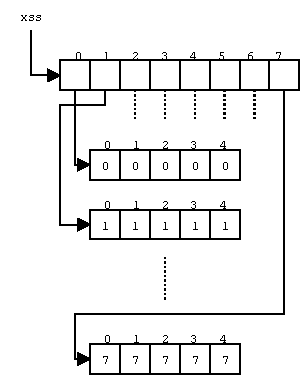
\includegraphics[scale=2]{chapters/figs/jaggedarrays.pdf}
  \caption{The memory representation of an 8 by 5 jagged array in \csharp{}.}
  \label{fig:jaggedarraydrawing}
\end{figure}


\texttt{xss} is an array of arrays, so \texttt{xss} is a reference to an array
in memory, which itself contains references to other arrays.
To retrieve the variable \texttt{some\_two}, we first follow the reference to
the array \texttt{xss} in memory. There we get the second element, which is a
reference to another array in memory. In this array, we read the third element,
which in this case is the 2 that we wanted.

\begin{figure}[h]
  \centering
\begin{minted}{fsharp}
let i = 8
let j = 5
let xss = Array.init i <| (Array.create j) 
  
(* xss = [|
           [|0;0;0;0;0|];
           [|1;1;1;1;1|];
           [|2;2;2;2;2|];
           [|3;3;3;3;3|];
           [|4;4;4;4;4|];
           [|5;5;5;5;5|];
           [|6;6;6;6;6|];
           [|7;7;7;7;7|];
         |]
*) 

let some_two = xss.[2].[3]

\end{minted}
  \caption{Initializing a jagged array of integers in FSharp}
  \label{fig:jaggedarrayfsharp}
\end{figure}

Denoting by $r$ the rank of the jagged array, the lookup requires $r$ 
queries to memory, because accessing an array requires a memory acces, 
and we have to follow $r$ references to get to our element. If we just 
wanted a reference to the second array in \texttt{xss}, we would be 
chasing the first reference to \texttt{arr}, and then return one of 
the references stored within.

\fsharp{} also offers actual multidimensional arrays, of up to 32 dimensions.
As opposed to jagged arrays, the elements of these multidimensional arrays are
stored contiguously in memory, and the entire array can therefore be accessed at
once, instead of chasing references like with the jagged array. Chasing
references may introduce cache misses which carries cache penalties and
therefore a slower performance.

However, using multidimensional arrays in \fshark{} would make it much harder to
implement \fshark{}s SOACs in the standard library. 
When we apply functions from \fsharp{}s \texttt{Array} module to a jagged
array, we treat the jagged array as an array of elements.\\
For example, this means that applying \texttt{Array.map f} to a two-dimensional
jagged array \texttt{xss} will apply \texttt{f} to each array referred to by
\texttt{xss}.\\\\
If on the other hand, we used \texttt{Array2D.map} to map f over a
two-dimensional multidimensional array, we would actually apply f to each
element in the multidimensional array, and not each row or column in the
multidimensional array.

Implementing SOACs for multidimensional arrays would require a significant
effort, as opposed to with jagged arrays, where most SOACs already had
equivalent or near-equivalent counterparts in the \fsharp{} library.

\section{Converting jagged arrays to Futhark's flat arrays,  and back again}
\label{sec:convertingarrays}
As mentioned in section \ref{csharpentries}, we cannot just pass jagged arrays
as arguments to the Futhark \csharp{} entry functions.
Instead, we must convert our jagged array into a flat array and an array of
integers, and pass these two objects as arguments instead.

In figure \ref{fig:jaggedtoflat} we see a three dimensional array that is being
flattened. The array has $n \times m \times k$ elements.
\\
First, we split the three dimensional array into $k$ two dimensional arrays. The
$k$ elements are sorted by their previous $k$-index.
\\
We then take each of the $k$ two dimensional arrays and split them into $k
\times m$ dimensions of $n$ elements each.
These $k \times m$ $n$-elements arrays are sorted by first by their $k$ index
(lowest first), and then by their $m$ index.

To reshape the flattened array, just follow the arrows backwards.

\begin{figure}[H]
  \centering
  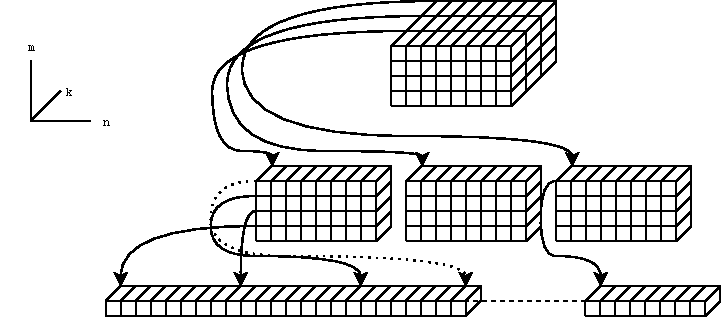
\includegraphics[scale=1.4, angle=270]{chapters/figs/jaggedtoflat.pdf}
  \caption{Flattening a three dimensional jagged array into one flat contiguous
    array.}
  \label{fig:jaggedtoflat}
\end{figure}

\subsection{Analysis of FlattenArray}
The simple algorithm for this flattening is described in pseudocode in figure
\ref{fig:flattenarray}. The implemented algorithm is slightly more complex, as
it has perform various type castings, and also checks for invalid arrays such as
irregular arrays.
In the example, the type $'b$ denotes a primitive type such as booleans or
integers. Type $a$ on the other hand, is any type variable \-- namely array
types.

\begin{figure}[h]
  \centering
\begin{minted}[linenos]{text}
FlattenArray (array : Array of a) : (Array of 'b * Array of int) =
  match typeOf(array) with
  | Array of 'b ->
    return (array, [len(array)])
  | Array of _ ->
    subarrays_and_lengths = map FlattenArray array
    (subarrays, subarrays_lengths) = unzip subarrays_and_lengths
    subarray_lengths = head(subarrays_lengths)
    concatenated_subarrays = concat subarrays
    this_length = len(array)
    lengths = [this_length] @ subarray_lengths
    return (contatenated_arrays, lengths)
\end{minted}
  \caption{Flattening jagged arrays, pseudocode}
  \label{fig:flattenarray}
\end{figure}

When FlattenArray first is called with a jagged array as input, we don't know
how many dimensions this array has. Therefore, we recursively call FlattenArray
on the subarrays of the arrays, until these recursive calls reach a base case.
The base case is the array that does not contain array references, but primitive
values.

\begin{description}
\item[\texttt{L2}]: For a one dimensional jagged array, this branch is taken once.
  For a jagged array of $d$ dimensions, it's taken
  $\prod_{n=1}^{d-1}(\text{subarrays at }d_n)$ times.

\item[\texttt{L3}] is the base case, which takes $O(1)$ time. This is because we
are just returning a tuple with the original array, and singleton array that holds the length of the
array (creating the singleton array is also $O(1).$)

\item[\texttt{L4}]:
  For a jagged array of $d$ dimensions, this branch is taken
  $\prod_{n=1}^{d-1}(\text{subarrays at }d_n)$ times.

\item[\texttt{L5}] is the start of the recursive case. This line is called
  $O(d)$ times, $d$ being the number of dimensions in the jagged array.
  The result of \texttt{map FlattenArray array} is an array of \texttt{a} array references
  and integer array references.

\item[\texttt{L6}] MORE HERE
\item[\texttt{L7}] simply retrieves a reference to the first array in the array
  of subarray lengths. This is $O(1)$.
\item[\texttt{L8}] is by far the most costly line in the function.
  \fsharp{}s \texttt{Array.concat} function takes a sequence of arrays,
  allocates a new array, and copies each element of the old arrays into the new array.
  Each of the $n$ elements in the jagged array is copied to a new array a maximum of $d$
  times, which means we are performing $O(n*d)$ reads and writes.
  
\item[\texttt{L9}] retrieves the length of an array, and is $O(1)$.

\item[\texttt{L10}] appends a singleton array to the accumulated array of
  subarray dimensions, by first creating a singleton array, and then copy both
  the single element and the contents of the accumulated array to a third array
  of their collected length.
\end{description}

All in all, the upper bound on the \texttt{FlattenArray} algorithm is $O(n*d)$.
This is a far cry from the performance of flattening in Futhark. Flattening is
done in $O(1)$, as flattening merely calculates the product of the dimensions of
the array, and returns the result as the new single dimension of the array.

\subsection{Analysis of UnflattenArray}
The algorithm \texttt{UnflattenArray} in figure \ref{fig:unflattenarray}
restores the flat array from the Futhark \csharp{} program, to a jagged array in \fsharp{}.

\begin{figure}[H]
  \centering
\begin{minted}[linenos]{text}
UnflattenArray (lengths : Array of int) (data : Array of a) =
  match len(lengths) with
  | 1 ->
    return data
  | _ ->
    length = head(lengths)
    lengths' = tail(lengths)
    data' = chunk_array length data 
    data'' = map (UnflattenArray lengths') data'
    return data''
\end{minted}
  \caption{Recreating a jagged array from flat array with dimensions}
  \label{fig:unflattenarray}
\end{figure}

Like in \texttt{FlattenArray}, the most expensive line in the function is the
array-manipulating one. In \texttt{UnflattenArray}, it is line 7: For each
dimension in the lengths array, we chunk our data array into multiple smaller
arrays. Each of the $n$ elements in the initial array is moved to a new and smaller array
$d$ times, which makes the complexity of this algorithm $O(n*d)$.

\subsection{Why UnflattenArray hinders a specific tuple type}
\label{subsec:hinderedtupletype}

When an \fshark{} function is invoked, it's arguments are prepared by an
argument converter first. For scalar arguments, the argument is simply returned.
But for array arguments, we must flatten the jagged array into a tuple that
follows Futhark's array representation.

When the Futhark function returns, we then have to unflatten the Futhark arrays
back into jagged arrays. To do this, we naively look at all the values
returned by the Futhark function, and whenever we encounter a tuple of type
\texttt{('a [] * int64 [])}, we assume that this is a flat array that needs to
be unflattened.
This procedure works fine, but has one side effect: \fshark{} doesn't support
entry functions that has (\texttt{('a [] * int64 [])}) tuples in their return
types, because this type is reserved.

To circumvent this, the user is instead encouraged to return the tuple as two
separate values.

\subsection{An alternative solution (FSharkArrays)}
Instead of using jagged arrays (or even multidimensional arrays), we initially
considered implimenting an \fshark{} specific array type, which could be directly
translated to Futhark's flat array structure.

This data type is shown in figure \ref{fig:fsharkarrays0}.
An {\tt FSharkArray<'a>} contains a flat array of {\tt <'a>}, and a list of integers
denoting the lengths of the arrays contained in the flat array.

\begin{figure}[H]
  \centering
\begin{minted}{fsharp}
type FSharkArray<'a> = class
  val mutable flatArray : 'a array 
  val mutable dimensions : int array
  end
\end{minted}
  \caption{The basic structure of an FSharkArray}
  \label{fig:fsharkarrays0}
\end{figure}

This would allow us to skip the flattening and unflattening algorithms that are
currently used for invoking imported Futhark functions, and instead just pass
the contents of the arrays \textit{as is}.

However, this approach was deemed impractical for several reasons.
Jagged arrays readily support getting subarrays and elements using the array
indexing operator intuitively. for example, for a two-dimensional array \texttt{xss :
  int [][]}, we can expect that \texttt{xss.[1]} returns a subarray, and that \texttt{xss.[1].[4]}
returns an integer. 
For example, to get the same functionality for \texttt{FSharkArrays}, we would have to implement the
array operator for \texttt{FSharkArrays} manually. The array operator would have
to access the flat array by calculating an offset using the array operator
operands together with the lengths stored in the \texttt{dimensions} integer
array.

Besides calculating array indexes manually, we would also have to handle that
the index operator must be able to return either an element of some type
\texttt{'a}, or another \texttt{FSharkArray}. This could be handled by
implementing \texttt{FSharkArray} as a discriminated union type instead; as
shown in figure \ref{fig:fsharkarrays1}.

\begin{figure}[H]
  \centering
\begin{minted}{fsharp}
type FSharkArray 'a = FlatArray of ('a array * int array)
                    | Element of 'a
\end{minted}
  \caption{FSharkArray as a discriminated union type}
  \label{fig:fsharkarrays1}
\end{figure}
This way, an \texttt{FSharkArray} can be either an array or an element. However,
we then have a third problem.
Wherever we are using \texttt{FSharkArray 'a}, our elements from the arrays will be wrapped as
\texttt{Element of 'a}s.

This means that we will have to either implement a custom set of \fsharp{}
operators and standard library functions which unwraps \texttt{Elements} before
passing them on to the actual operator or function, or at least implement an
unwrapper function of type $unwrap : Element~of~'a~\to~'a$, which must be applied
everywhere in functions that uses both \texttt{FSharkArrays} and \fsharp{}
standard library functions.

\subsection{Conclusion on arrays}
Ultimately, choosing between jagged arrays, multidimensional arrays and
FSharkArrays became a question of simplicity vs. performance.
For \fshark{}, I had the liberty to focus solely on simplicity, as \fshark{}
code is neither intended or even efficient when executed as native FSharp code.
Therefore I could choose to let \fshark{} use jagged arrays, instead of any of
the other options.

The syntax for declaring a jagged array type closely
resembles Futhark's multidimensional array syntax (take for instance FSharp's
\texttt{int[][]} versus Futhark's \texttt{[][]i32} for declaring
two-dimensional integer arrays).
The close similarities between Futhark and \fshark{} code means that \fshark{}
generated Futhark code is easier to read for debugging purposes, and likewise
makes Futhark code easier to port to \fshark{}.

%%% Local Variables:
%%% mode: latex
%%% TeX-master: "../thesis"
%%% End:
